\section{Part I. Problem Setup}
\subsection{Task 1.1}
\textit{Calculate the necessary inlet velocity, $U_\infty$, so that the Reynolds number ($\text{Re} = U_\infty D/\nu$) of 3000 is achieved. Assume the inlet Turbulence Intensity at 1\%.}

The working fluid is air. The properties of air at 15$^\circ$C are
\begin{align*}
    \rho &= 1.225 \text{ kg/m}^3 \\
    \eta &= 1.7894 \times 10^{-5} \text{ Pa s} 
\end{align*}
The required inlet velocity is then
\begin{align*}
    U_\infty &= \frac{\text{Re} \eta}{\rho D_h} \\
    &= \frac{\text{Re} \eta}{\rho 2h} \\
    &= \frac{3000 \times 1.7894 \times 10^{-5}}{1.225 \times 2 \times 0.0052} \\
    &= \boxed{4.21 \text{ m/s}}
\end{align*}

\section{Part II. Reference Simulation}
\subsection{Task 2.1}
The simulation was carried out. The residuals are shown in Figure \ref{fig:residuals plot}
\begin{figure}[H]
    \centering
    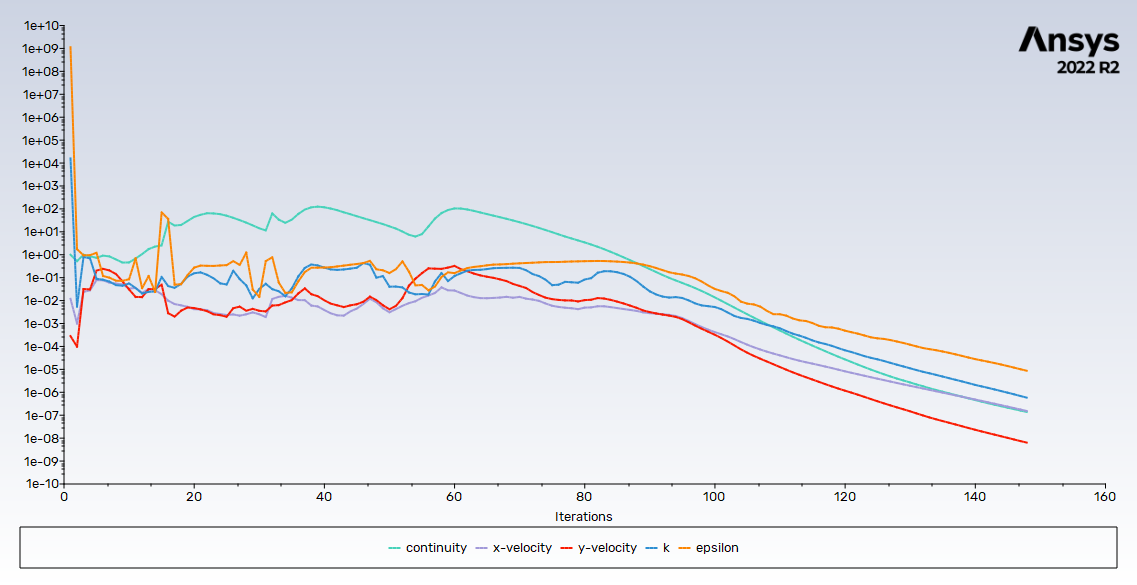
\includegraphics[width=0.8\textwidth]{Questions/Figures/Residuals.png}
    \caption{Residuals for the $k-\epsilon$ model}
    \label{fig:residuals plot}
\end{figure}

\subsection{Task 2.2}
\subsubsection{I)}
\textit{Plot the monitor point data (Pressure, Velocity Components and Turbulence Intensity) at $P_1$ as a function of iteration number. Have we reached convergence? Why? Justify your answer.}
\begin{figure}[H]
    \centering
    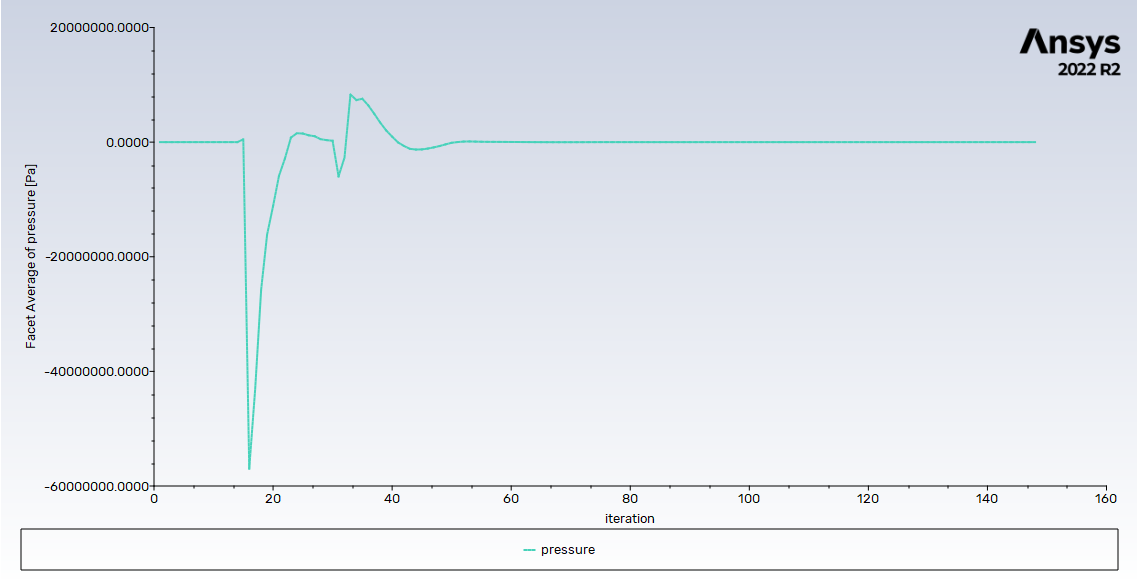
\includegraphics[width=0.8\textwidth]{Questions/Figures/Pressure at point.png}
    \caption{Pressure at $P_1 = (h, h, 0)$ over iterations}
\end{figure}
\begin{figure}[H]
    \centering
    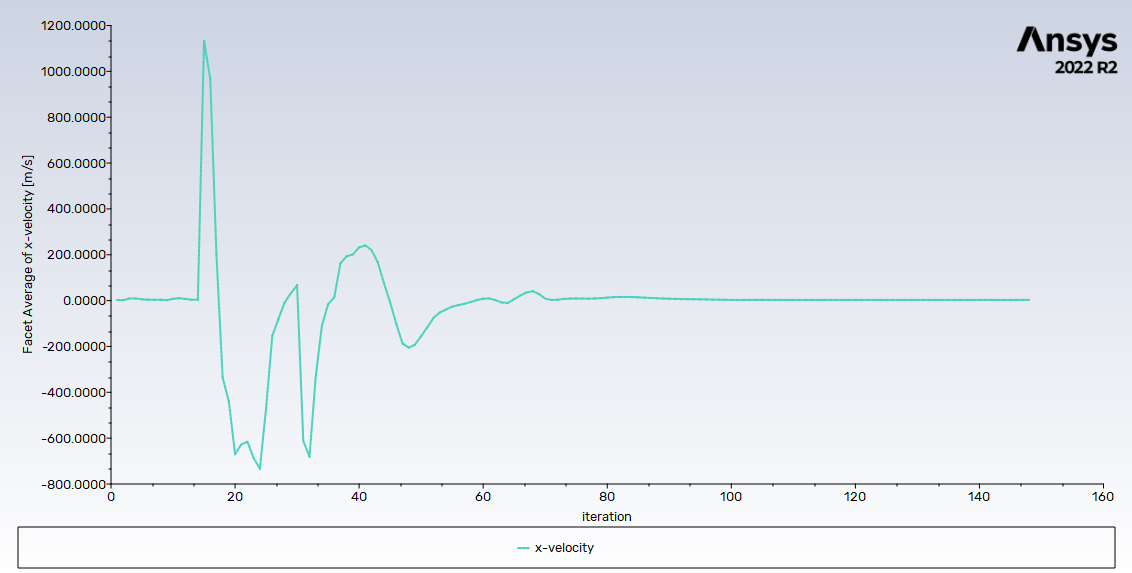
\includegraphics[width=0.8\textwidth]{Questions/Figures/x velocity at point.png}
    \caption{Streamwise velocity at $P_1 = (h, h, 0)$ over iterations}
\end{figure}
\begin{figure}[H]
    \centering
    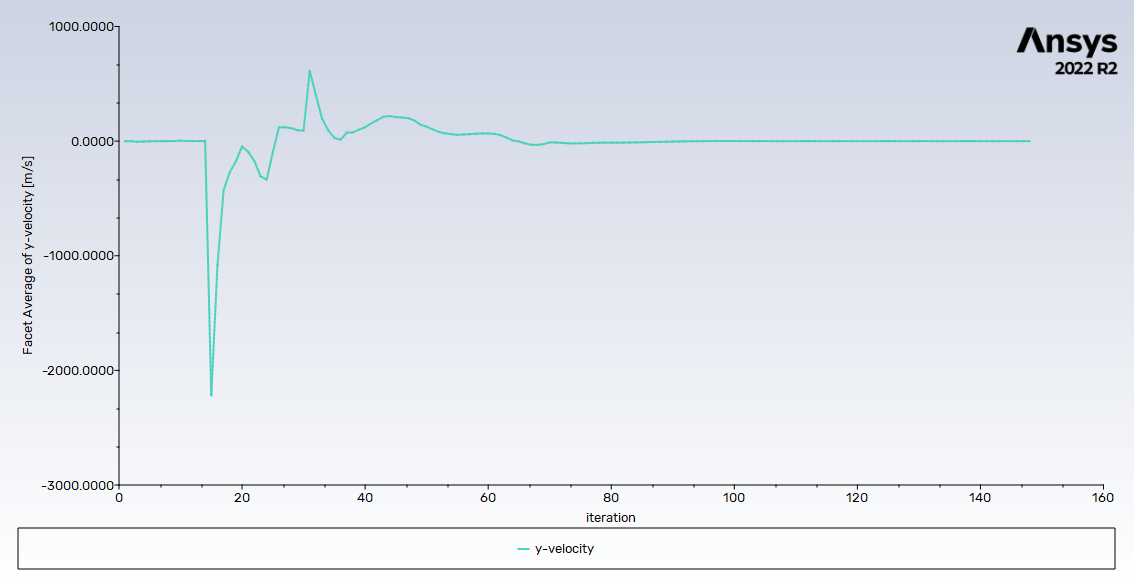
\includegraphics[width=0.8\textwidth]{Questions/Figures/y velocity at point.png}
    \caption{Spanwise velocity at $P_1 = (h, h, 0)$ over iterations}
\end{figure}
\begin{figure}[H]
    \centering
    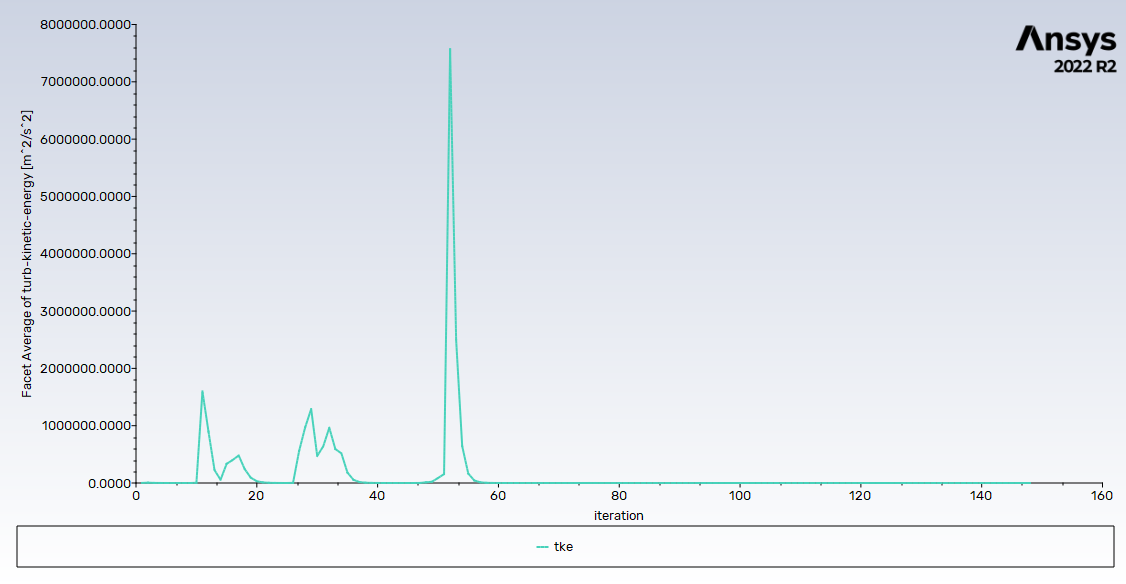
\includegraphics[width=0.8\textwidth]{Questions/Figures/Tke at point.png}
    \caption{Turbulence kinetic energy at $P_1 = (h, h, 0)$ over iterations}
\end{figure}
Convergence has been reached as all quantities have reached a steady state value. Though it is difficult to see because of the large spike in the first few iterations, upon reviewing the .dat files, it is clear that the values have converged.

\subsubsection{II)}
\textit{Create a contour plot of mean pressure ($p$) on the xy-plane. Adjust the values of maximum and minimum pressure so that the recirculation vortex is distinguishable from the flow.}
\begin{figure}[H]
    \centering
    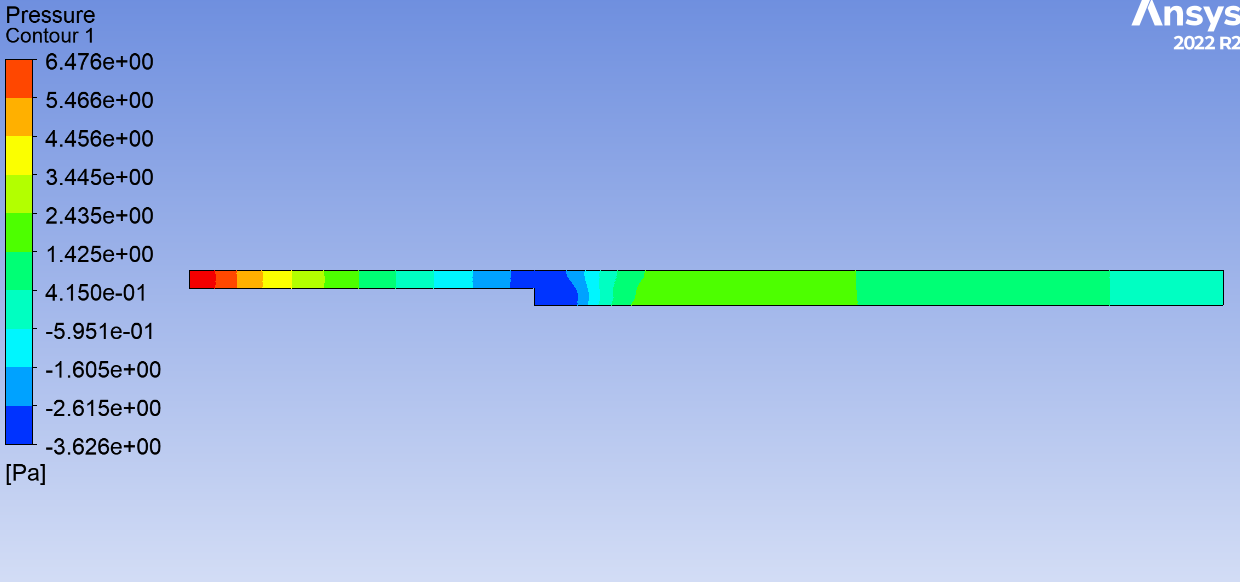
\includegraphics[width=0.8\textwidth]{Questions/Figures/pressure contour.png}
    \caption{Mean pressure contour on the xy-plane}
\end{figure}

\subsubsection{III)}
\textit{Create a contour plot of Turbulent Kinetic Energy ($k$) on the xy-plane. Adjust the values of maximum and minimum values of $k$ so that turbulent structures are apparent in the flow.}
\begin{figure}[H]
    \centering
    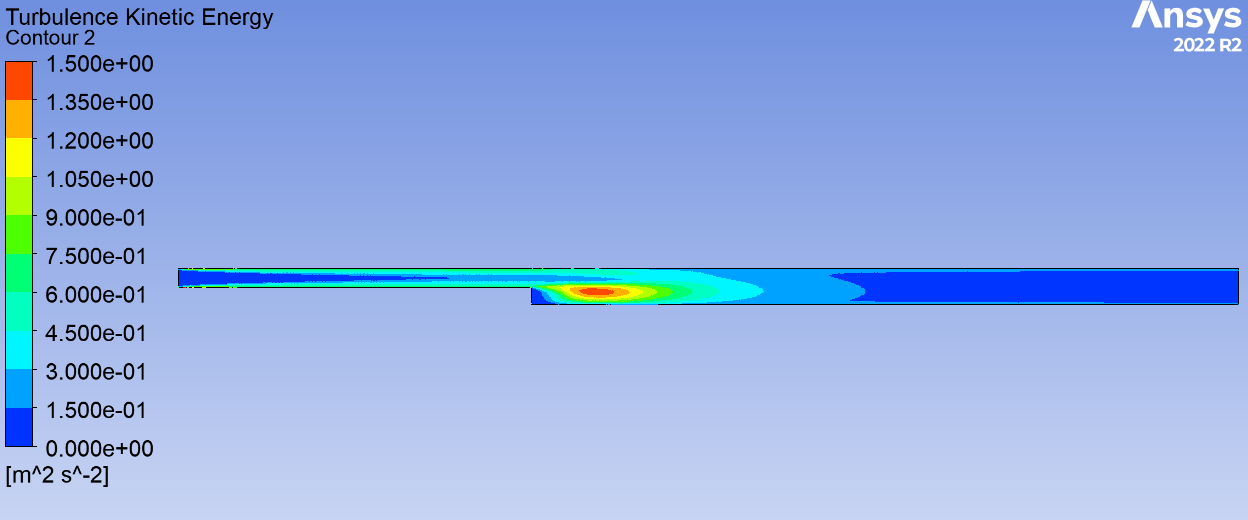
\includegraphics[width=0.8\textwidth]{Questions/Figures/tke contour.png}
    \caption{Turbulent kinetic energy contour on the xy-plane}
\end{figure}

% Create a contour plot of spanwise vorticity (ωZ) on the xy−plane. Adjust the values of
% maximum and minimum vorticity so that the vortex shedding is distinguishable from
% the flow.
\subsubsection{IV)}
\textit{Create a contour plot of spanwise vorticity ($\omega_z$) on the xy-plane. Adjust the values of maximum and minimum vorticity so that the vortex shedding is distinguishable from the flow.}
\begin{figure}[H]
    \centering
    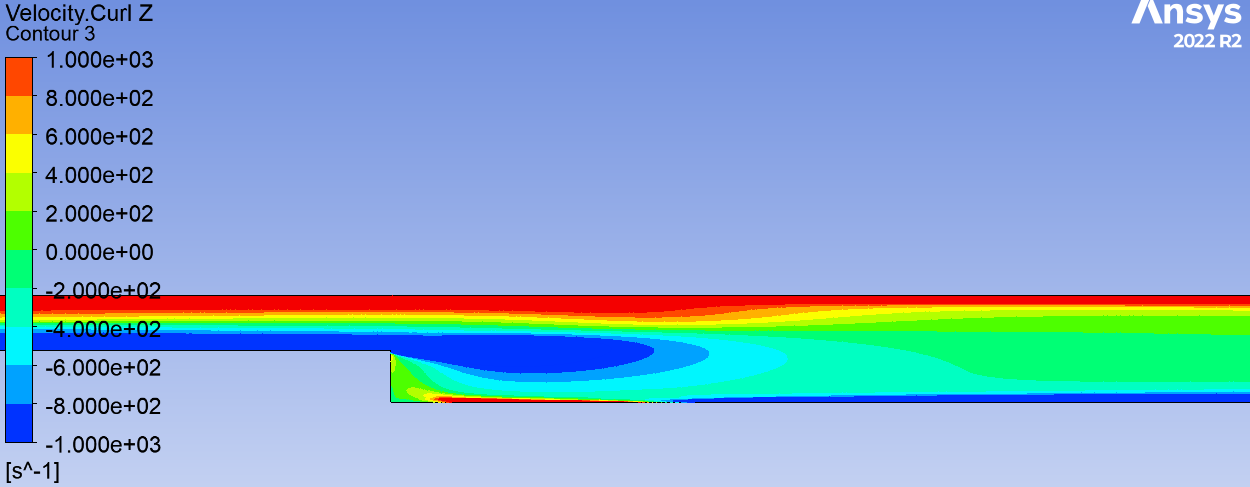
\includegraphics[width=0.8\textwidth]{Questions/Figures/vorticity contour.png}
    \caption{Spanwise vorticity contour on the xy-plane}
\end{figure}

\subsubsection{V)}
\textit{Draw the profile of mean streamwise ($x$-direction) velocity ($u$) along a horizontal line at $y = 0.5$ mm, and calculate the normalized value of $L_r$, which is the mean recirculation length of the step vortex. Normalize the plot using $h$.}

\begin{figure}[H]
    \centering
    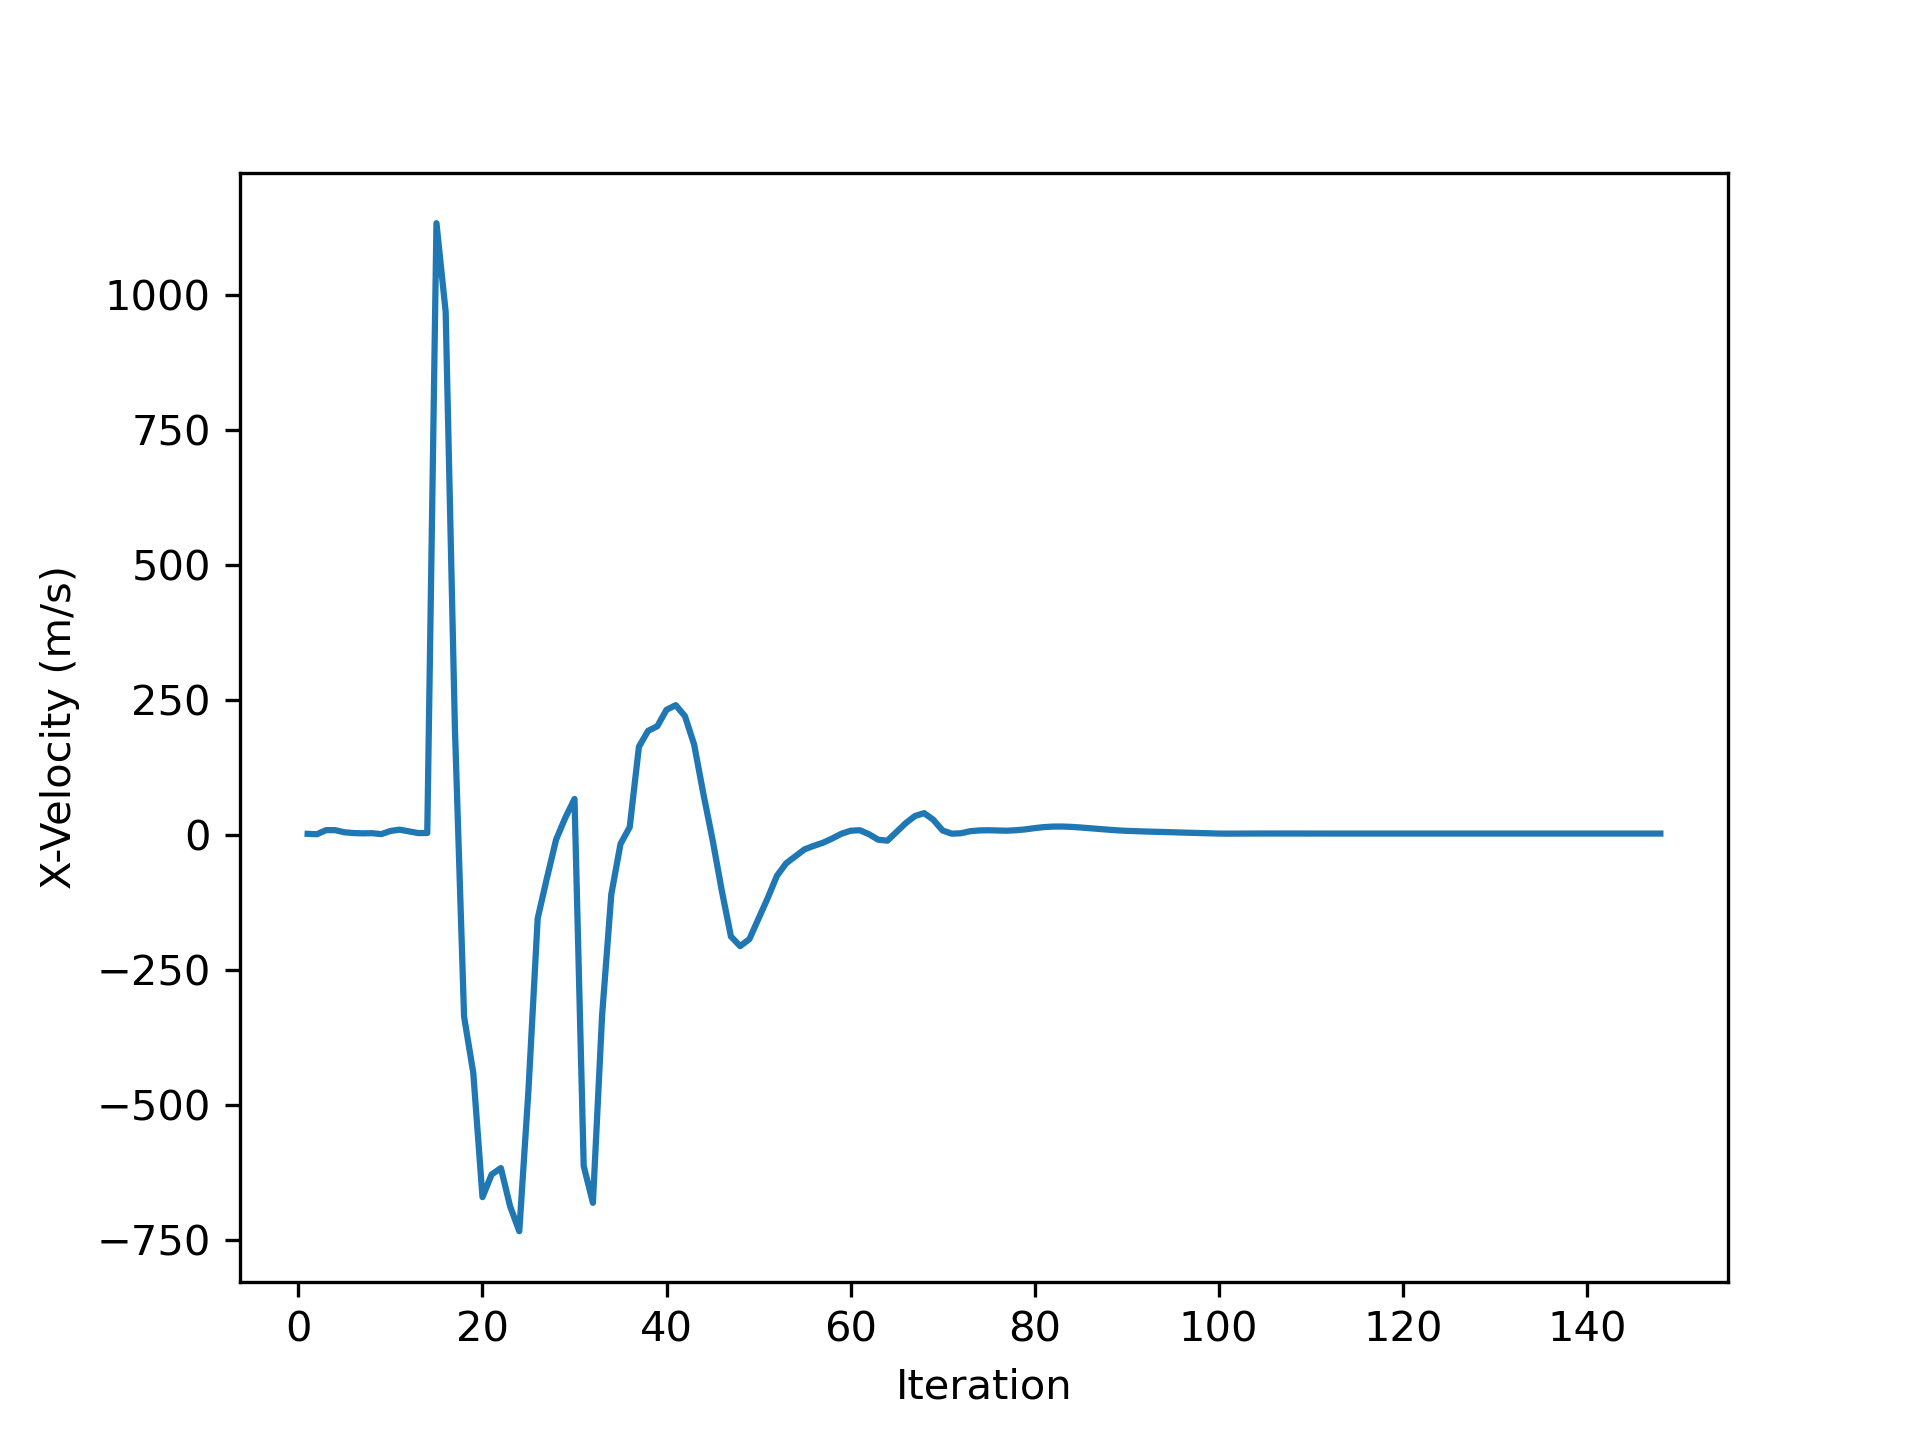
\includegraphics[width=0.8\textwidth]{Questions/Figures/X-Velocity.png}
    \caption{Mean streamwise velocity along a horizontal line at $y = 0.5$ mm}
\end{figure}
\begin{figure}[H]
    \centering
    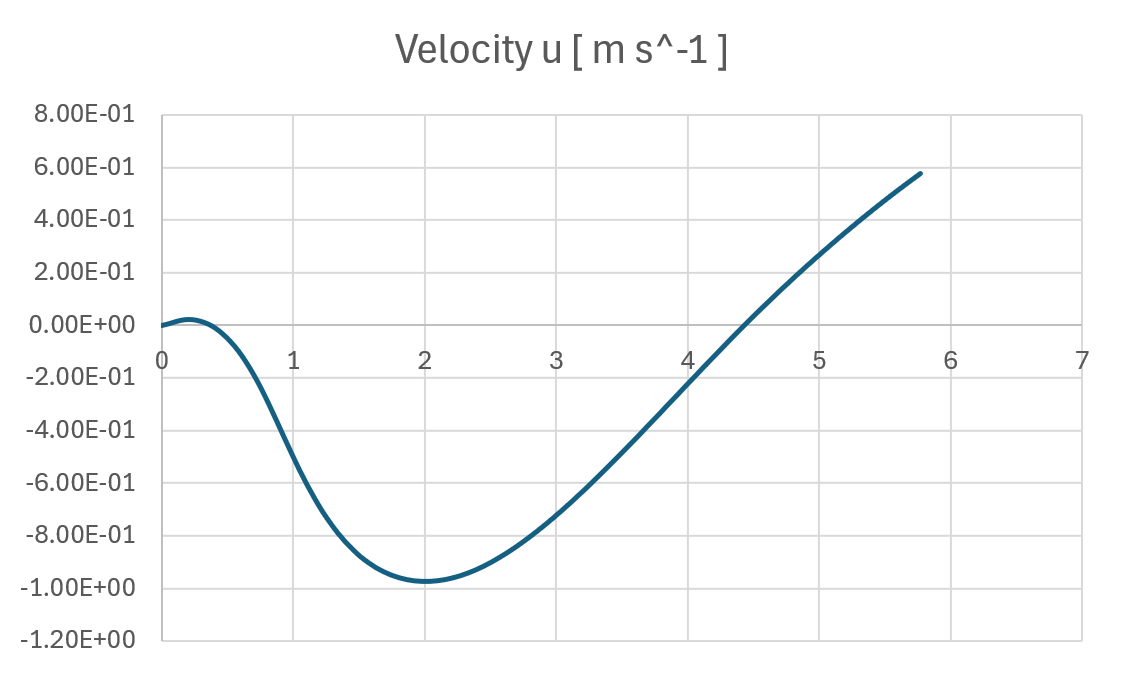
\includegraphics[width=0.8\textwidth]{Questions/Figures/Normalized x-velocity.png}
    \caption{Normalized mean streamwise velocity along a horizontal line at $y = 0.5$ mm}
\end{figure}
The recirculation length is approximately
\begin{align*}
    \hat{L}_r &= \frac{\Delta x}{h} \\
    &= \frac{2.30 \times 10^{-2} - 1.82 \times 10^{-3}}{0.0052} \\
    &= \boxed{4.073}
\end{align*}

\subsubsection{VI)}
\textit{Draw the profile of Turbulence Kinetic Energy (k) along the same horizontal line. Normalize the plot using $h$ and $U_\infty$.}
\begin{figure}[H]
    \centering
    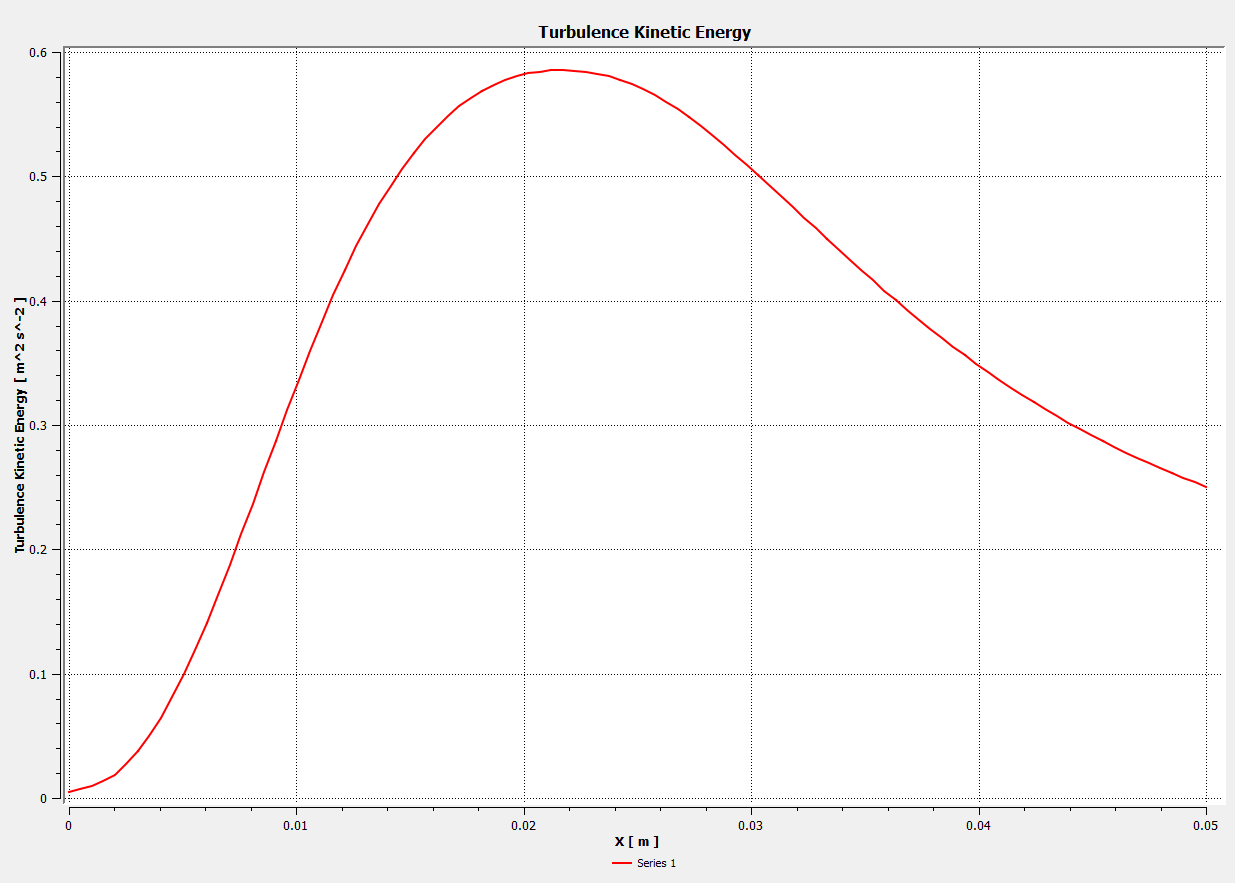
\includegraphics[width=0.8\textwidth]{Questions/Figures/tke along line plot.png}
    \caption{Turbulence kinetic energy along a horizontal line at $y = 0.5$ mm}
\end{figure}
Unfortunately I forgot to export the raw data. If I had the raw data, then I would've done
\begin{align*}
    \hat{k} &= \frac{k}{h U_\infty^2}
\end{align*}

\subsubsection{VII)}
\textit{Create a plot of flow streamlines (use Velocity as the parameter) on the xy-plane (Sides boundary). Adjust the number of streamlines so that the recirculating vortex is visible after the step. (You need to select Surface Streamlines and choose the Sides boundary as your surface. Overlay the contour plot of Velocity $u$ on the streamline plots, so that the recirculating vortex is identifiable.)}
\begin{figure}[H]
    \centering
    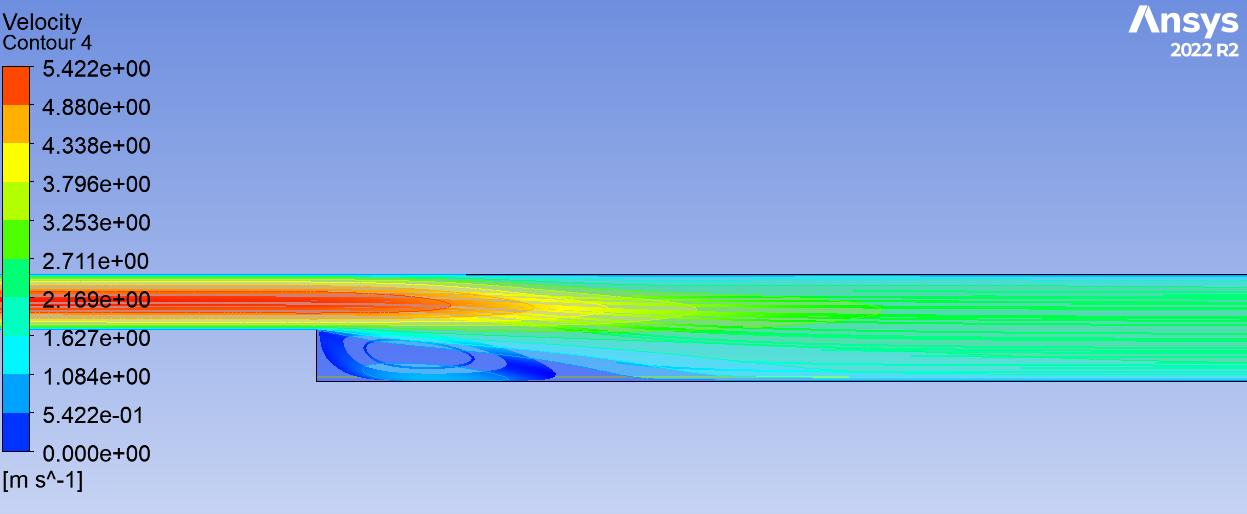
\includegraphics[width=0.8\textwidth]{Questions/Figures/streamlines plots.png}
    \caption{Flow streamlines on the xy-plane}
\end{figure}

\subsection{Task 2.3}
\textit{Discuss the relationship between Turbulent Kinetic Energy and the location of flow structures. Are there a correlation? What does that mean?}
The relationship between Turbulent Kinetic Energy and flow structures can be observed through various locations in the flow. TKE tends to peak in specific regions, such as the recirculation zone, wake of the step, and shear layer. This is because these areas typically involve either decelerating or accelerating flow, which leads to the generation of turbulence.

In the recirculation region, where flow is slowing down, TKE is naturally high as turbulence is being generated. Similarly, in the wake of the step, where flow decelerates, TKE levels are also elevated due to turbulence generation.

\section{Part III. Post-Processing Using Tecplot}
\subsection{Task 3.12}
\begin{figure}[H]
    \centering
    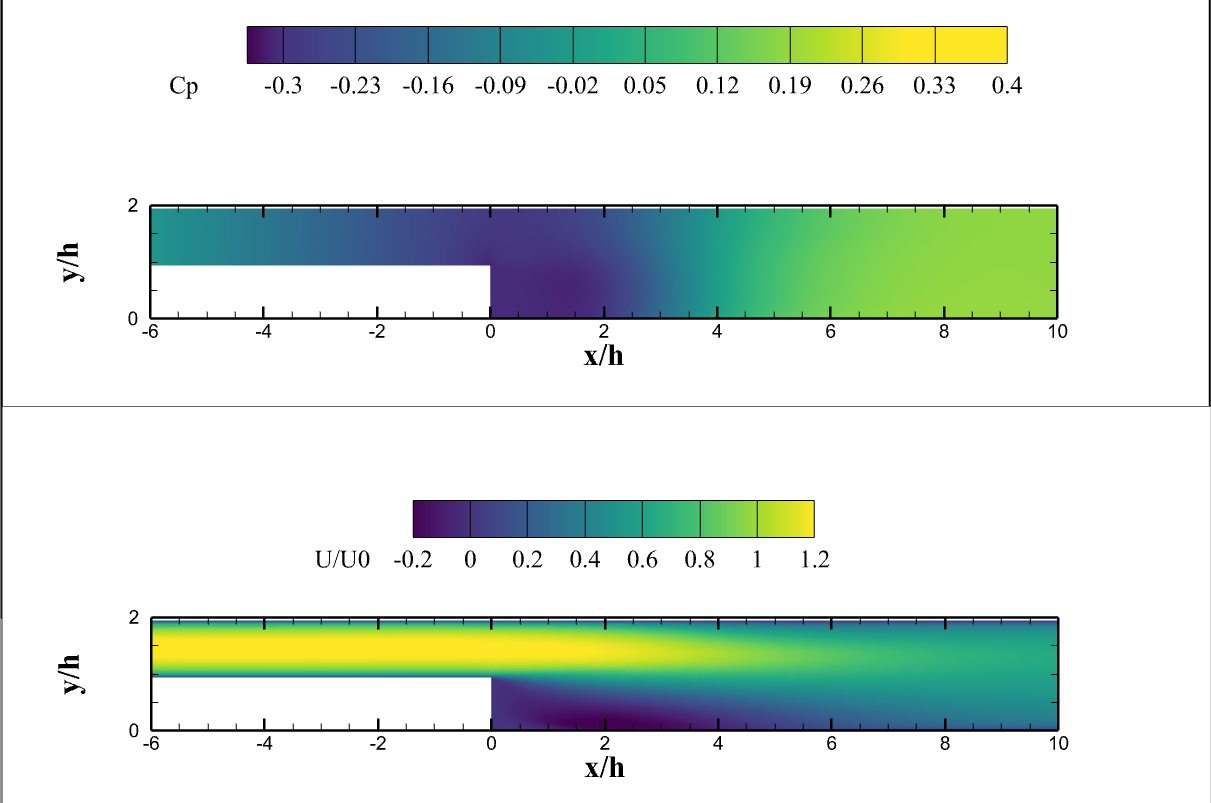
\includegraphics[width=0.8\textwidth]{Questions/Figures/tecplot.png}
    \caption{Pressure contour on the xy-plane using Tecplot}
\end{figure}